% PACKAGES INCLUDED HERE 
% DO NOT NEED TO CHANGE
\documentclass[conference]{IEEEtran}
%\IEEEoverridecommandlockouts
% The preceding line is only needed to identify funding in the first footnote. If that is unneeded, please comment it out.
\usepackage{cite}
\usepackage{amsmath,amssymb,amsfonts}
\usepackage{algorithmic}
\usepackage{graphicx}
\usepackage{textcomp}
\def\BibTeX{{\rm B\kern-.05em{\sc i\kern-.025em b}\kern-.08em
    T\kern-.1667em\lower.7ex\hbox{E}\kern-.125emX}}
\begin{document}

% TITLE GOES HERE

\title{Image Captioning\\}


% AUTHOR NAMES GOES HERE

\author{\IEEEauthorblockN{1\textsuperscript{st} Zernab Saeed}
\IEEEauthorblockA{\textit{Department of Computer Science} \\
\textit{Middle Tennessee State University}\\
Murfreesboro, TN USA \\
zs2s@mtmail.mtsu.edu}
\and
\IEEEauthorblockN{2\textsuperscript{nd} Alejandro Lopez}
\IEEEauthorblockA{\textit{Department of Computer Science} \\
\textit{Middle Tennessee State University}\\
Murfreesboro, TN USA \\
asl3u@mtmail.mtsu.edu}
\and
\IEEEauthorblockN{3\textsuperscript{rd} Daniel Sindell}
\IEEEauthorblockA{\textit{Department of Computer Science} \\
\textit{Middle Tennessee State University}\\
Murfreesboro, TN USA \\
ds8h@mtmail.mtsu.edu}
\and

\IEEEauthorblockN{4\textsuperscript{th} Pratap Karki}
\IEEEauthorblockA{\textit{Department of Computer Science} \\
\textit{Middle Tennessee State University}\\
Murfreesboro, TN USA\\
pk3j@mtmail.mtsu.edu}
\and
\IEEEauthorblockN{5\textsuperscript{th} Michael Kwarteng}
\IEEEauthorblockA{\textit{Department of Computer Science} \\
\textit{Middle Tennessee State University}\\
Murfreesboro, TN USA \\
mak5z@mtmail.mtsu.edu}

}


\maketitle

% ABSTRACT 

\begin{abstract}
The integration of Neural Networks in everyday technology is growing exponentially. Caption generation is the challenging artificial intelligence problem of generating a human-readable textual description given a photograph. It requires both understanding from the domain of computer vision and a language model from the field of natural language processing. Our objective is to utilize the already available research and leverage the tools we use in class to learn how to build a deep learning Neural Network that generates a caption after analyzing an image.  We looked into different approaches to this task and decided to use the Encoder-Decoder Architecture to build the network. To feed the model, we prepared data from the ImageNet data collection. The Xception, a pre-trained Convolutional Neural Network that extracts picture features from our dataset, serves as the encoder's output layer. We concatenated this model with an Long- Short Term Memory layer that acts as a decoder which will decode the vector representation into the corresponding output sequence using another recurrent hidden layer.  Due to delays, our findings and testing methods are insufficient and do not represent the entirety of the project. We want to keep working on our model to train it and experience the outcomes we envisioned while learning from our mistakes.
\end{abstract}


% KEYWORDS

\begin{IEEEkeywords}
CNN, LSTM, Encoder, Decoder
\end{IEEEkeywords}

% INTRODUCTION SECTION
\section{Introduction}

Neural Networks are computer systems that simulate human brain function. They are made up of interconnected parallel processing components that collaborate to solve problems and make connections by "learning" rather than memorizing. They are taught to identify new data sets by making correlations between what they have already learned, just like the human brain. Because of the widespread availability of increasingly advanced technologies, practitioners may now experiment with neural network-based training methods that were previously thought to be too difficult to implement. This concept of using a deep learning neural network to process and understand a scene in an image and then producing a caption has many applications, including the realization of human-computer interaction. 

Our project reflects an interpretation of what we wanted our model to do and what we hoped to achieve, rather than a full trained and high accuracy depiction of an Image Captioning Neural Network. We prepared data using the ImageNet dataset containing 100 images, which we had studied in class. We used a pre-trained model, the ImageNet Xception model, to pre-compute photo features, which converts images into an encoding that can be interpreted by a computer, after preparing this data. The Xception model is a Convolutional Neural Network that has been pretrained on the ImageNet database with python and Keras deep learning. The feature extraction base of the Xception architecture consists of 36 convolutional layers \cite{b1}. The Xception Model outperformed any other ImageNet architecture such as VGG16 and Inception. The experiments that highlighted the accuracy and performance of the Xception model, as well as our familiarity with it aided in the decision to use this model. To prevent the network from interpreting the images, we removed the top layer. The sequence from the text was then processed, a feature vector was extracted, and the output was decoded using an LSTM and Dense layer.

% CREATES IMAGE FIGURE
\begin{figure}[htbp]
\centerline{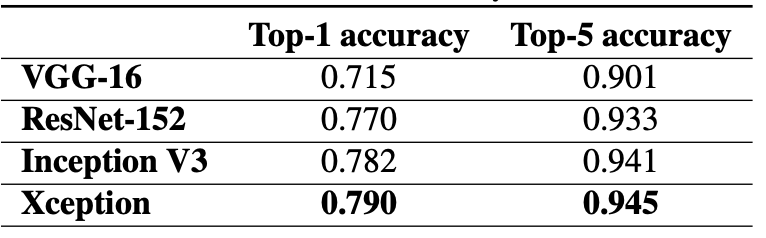
\includegraphics[width=\linewidth]{comaprenets.png}}
\caption{Xception net performance.}
\label{fig1}
\end{figure}

Our project was driven and based off of tutorials and implementations from the following references: \cite{b2} \cite{b3} \cite{b4}

% BACKGROUND SECTION
\section{Background}

Automatically describing the content of an image using properly constructed English sentences is a difficult task, but it could have a significant effect, such as assisting visually disabled people in better understanding the content of web images. Image Captioning is useful when it can identify objects and relations of objects in an image. Not only is it difficult to prepare data on text files because semantic information must be conveyed, but a language model is also needed to complete this task \cite{b5}. Our main motivation for this project stems from our desire to learn more about Neural Networks and to practically implement core concepts introduced to us in class. Even though object recognition has seen a lot of progress, automatically defining the contents of images is still a difficult task, even more difficult than visual classification. Image captioning models must provide a detailed understanding of a given image in order to capture the complex relationships between objects and identify the most important ones. Furthermore, they must comprehend image-language interactions and convert image representations into language representations. Finally, the sentences generated to express the captured information need to be natural \cite{b6}.  

The encoder-decoder model seemed to resonate with us among the various types of architectures we investigated. A convolutional neural network (CNN) is typically used as the encoder, while a recurrent neural network is used as the decoder (RNN). The encoder uses a vector to represent the image, capturing objects and semantic information, while the decoder uses the image representation to produce natural sentences. However, it's unlikely that this vector can capture all of the structural data required to generate the definition in the subsequent decoding process.Furthermore, decoder steps must produce sentences that both explain the contents of the picture and match the trained language model. To use an encoder-decoder model to caption an image, we must first transfer the image through a Convolutional Network and remove the last output layer. Removing the last layer prevents the network for interpreting images. 

A sequence model that generates text is concatenated with the final layer. The start token, which will signal the start of a sentence, is used to categorize data sent through the LSTM. To do so, an image will be submitted to a pretrained CNN, which will extract photo features from the images and transform them into a vector. The CNN's vector output will be sent through another linear layer that will map the size of the output vector to the size of the LSTM layer's input vector \cite{b7}.

A major question for Machine Learning is how to learn such good features automatically \cite{b8}. A Convolutional Neural Network (CNN) is a Deep Learning algorithm that attempts to solve this problem by taking an input image and assigning weights and biases that are most efficient at learning various aspects/objects in the image, as well as distinguishing images one from the other. The architecture of a CNN is inspired by the organization of the Visual Cortex and is similar to the connectivity pattern of Neurons in the Human Brain. Convolutional layers, non-linearity layers, pooling layers, and completely linked layers are all present in CNNs. The convolutional and fully- connected layers have parameters but pooling and non-linearity layers don't have parameters. The CNN has an excellent performance in machine learning problems \cite{b8}.

Convolutional Neural Networks learn internal feature representations from small squares of input data and expect and maintain the spatial relationship between pixels. Objects in the images can be moved or converted in the scene and still be detected by the network since features are learned and used across the entire image. 
This is why the network is so effective at recognizing objects in images, such as digits, names, and names in a variety of orientations. It has been demonstrated over the last few years that CNNs can provide a rich representation of an input image by embedding it in a fixed-length vector, which can then be used for a variety of vision tasks.
As a result, it makes sense to use a CNN as an image "encoder" by first pre-training it for an image classification task and then feeding the last hidden layer to the RNN decoder that generates sentences \cite{b9}. 

(https://arxiv.org/pdf/1411.4555.pdf) The ‘Xception,' a convolutional neural network architecture that relies solely on depth wise separable convolution layers, is the CNN we used in our project. The Xception architecture is a depth-wise separable convolution layer stack with residual connections. This makes it very simple to define and change the architecture \cite{b10}.

The LSTM is the base model that is used to predict caption sequences from feature vectors obtained from CNN. A RNN serves as the LSTM layer. Recurrent neural networks (RNNs) have cycles feeding the activations from previous time steps as input to the network to make a decision for the current input, unlike feedforward neural networks (FFNNs). The activations from the previous time step are stored in the internal state of the network and they provide indefinite temporal contextual information in contrast to the fixed contextual windows used as inputs in FFNNs. As a result, rather than a static fixed size window over the sequence, RNNs use a dynamically shifting contextual window of all sequence history. RNNs are best suited for sequence modeling tasks like sequence prediction and sequence labeling because of this capability \cite{b11}. In this case, the LSTM layer will serve as a decoder, decoding the vector representation into the corresponding output sequence with the help of another recurrent hidden layer. During preparation, special start and stop patterns are used to encode for the beginning and stopping points of goal sequences.

Image Captioning tasks are much harder because they require extensive text preparation. Text cleaning for descriptions is challenging because of the extensive amount of noise not visible to the trained eye. Text cleaning includes the process of loading the data, splitting it to get important information and removing punctuation. This includes tokenizing vocabulary, which deals with getting rid of words that are not useful in training the model and keeping alphabetical tokens. Identifying stop words which are not useful in captioning are also filtered out. 

We tried to be avid and create our own text description for the ImageNet dataset. This was a reasonable dataset given the time we had left due to setbacks and lack of communication in earlier stages of development. Our aim wasn’t to produce a perfect working model, rather it was to develop a deeper understanding of Neural Networks and explore the practical implementations of that knowledge. 


## % METHODS SECTION
\section{Methods}

\subsection{Architecture Overview}

The architecture that we have been describing thus far is the encoder-decoder architecture. This is a machine translation architecture in which an encoder network encodes an input sequence as a fixed-length vector. The encoding is then interpreted by a different decoder network, which produces an output sequence in the new language. The advantage of this approach, aside from its impressive abilities, is that it can be trained on the problem with a single end-to-end model. When adapted for image captioning, the encoder network is a deep convolutional neural network, and the decoder network is a stack of LSTM layers \cite{12}.

% CREATES IMAGE FIGURE
\begin{figure}[htbp]
\centerline{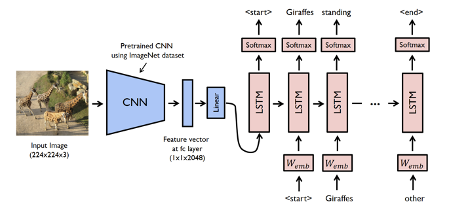
\includegraphics[width=\linewidth]{architecture.png}}
\caption{Visual understanding of model}
\label{fig}
\end{figure2}

\subsection{Data and Data Preparation}
The most crucial lesson we learned was how to prepare data for processing. We miscalculated the difficulty of data processing. The Flickr8k dataset was used in all of the image captioning models we saw. This data set was initially used to clarify our interpretation of what was going on and to learn how to prepare data. We then turned to the ImageNet dataset, which contained 100 images, which we had used in our Neural Nets class. This is a small dataset, but our goal wasn't to train a model to 100% accuracy; instead, we wanted to learn the fundamentals of how to create an Image Captioning Model. What we were missing from this dataset was the text that described each image. We decided to create our own text file of captions for each image. Each description corresponds to a unique image, which was used to identify and map descriptions to corresponding images. 

% CREATES IMAGE FIGURE
\begin{figure}[htbp]
\centerline{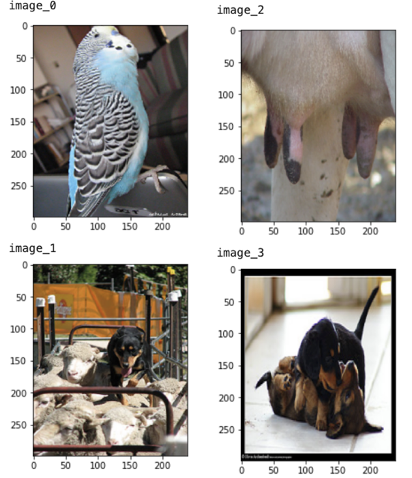
\includegraphics[width=\linewidth]{sampleimages.png}}
\caption{Example of images in Dataset}
\label{fig3}
\end{figure}

% CREATES IMAGE FIGURE
\begin{figure}[htbp]
\centerline{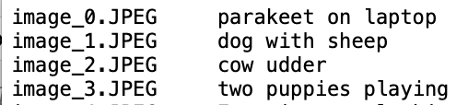
\includegraphics[width=\linewidth]{sampletext.png}}
\caption{Descriptions in textfile.}
\label{fig4}
\end{figure}

We cleaned up our image descriptions after loading the textfiles by writing functions that performed multiple tasks. We cleaned the data by separating the definitions into useful data and eliminating punctuation and newline characters. We tokenized and created a vocabulary that was simple to read and understand.After loading the definitions, we had to map them to the images and add specific terms or tokens like "startseq" and "endseq" to mark the beginning and end of each sentence. Our vocabulary had grown to 171 words after this data preparation. The figure depicts the most commonly extracted terms. 

% CREATES IMAGE FIGURE
\begin{figure}[htbp]
\centerline{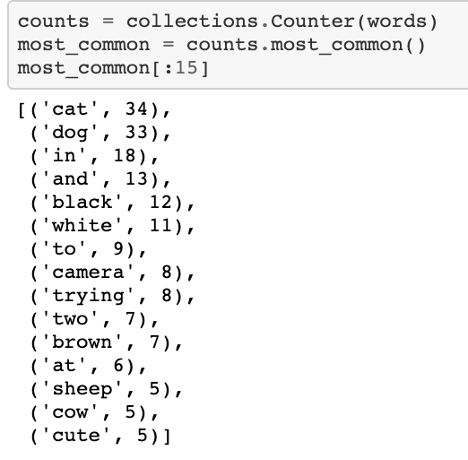
\includegraphics[width=\linewidth]{samplevocab.png}}
\caption{Example of vocabulary}
\label{fig5}
\end{figure}

The descriptions and potential captions before training contain our start and stop words. These words are essential and will help our LSTM layer identify when to start sequence processing. 

% CREATES IMAGE FIGURE
\begin{figure}[htbp]
\centerline{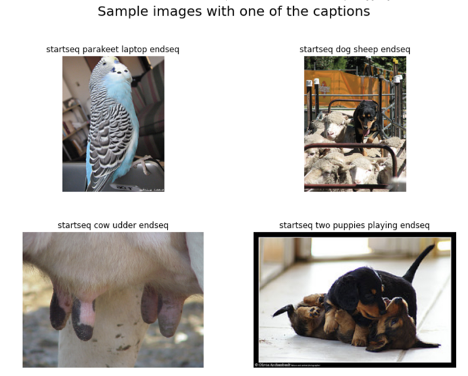
\includegraphics[width=\linewidth]{samplecaptions.png}}
\caption{Example of generated captions we expect}
\label{fig6}
\end{figure}

\subsection{Feature Exraction with Encoder}
After text and data has been prepared, we started to work on the model. We used a pre trained Xception Model to interpret the contents of the images. We use this model to pre-compute photo features which is an optimization that saves us time and memory. We used a one-to-one sequence prediction model that uses recursive calls to produce the textual summary. The single word input may be a token or the start of a sequence. The input word is integer encoded and then passed through a word embedding after the image has gone through a feature extraction model. To allow the model to predict the probabilities of words across the entire vocabulary, the output word is one hot encoded. The process of generating recursive words is repeated until an end-of-sequence token is produced \cite {b13}. 

% CREATES IMAGE FIGURE
\begin{figure}[htbp]
\centerline{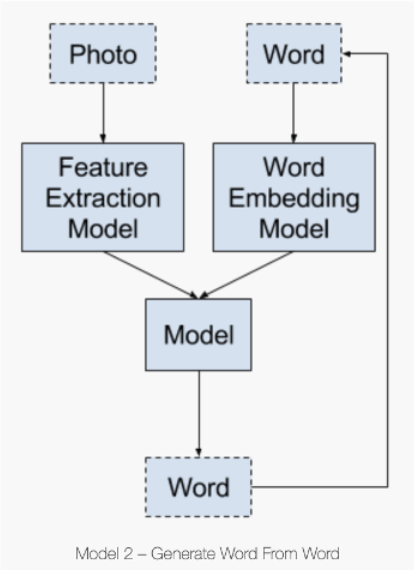
\includegraphics[width=\linewidth]{cnnmodel.png}}
\caption{Visualized working of model}
\label{fig7}
\end{figure}

Next we have the feature Extraction Model. The feature extraction model is a neural network that given an image, is able to extract the salient features, often in the form of a fixed-length vector. The feature extraction submodel is a deep convolutional neural network, or CNN. This network can be trained directly on the images in the image captioning dataset. The Xception model extracted features from the dataset and presented it in the form of a vector \cite {b14}.

\subsection{Generating Captions using Decoder}
A language model, in general, predicts the likelihood of the next word in the sequence based on the words already in the sequence.
The language model for image captioning is a neural network that, provided the network's extracted features, can predict the sequence of words in the description and build up the description based on the words that have already been created. A recurrent neural network, such as a Long Short-Term Memory network, or LSTM, is commonly used as a language model. In the series, each output time step generates a new term. According to our findings, LSTM reduces the issue of overfitting and tuning hyper parameters, while dropout improves model accuracy. Each generated word is then encoded using a word embedding and passed to the decoder as input to generate the next word. The language model can be trained independently using pre-computed image dataset features, in conjunction with the feature extraction network, or in any combination. 

% CREATES IMAGE FIGURE
\begin{figure}[htbp]
\centerline{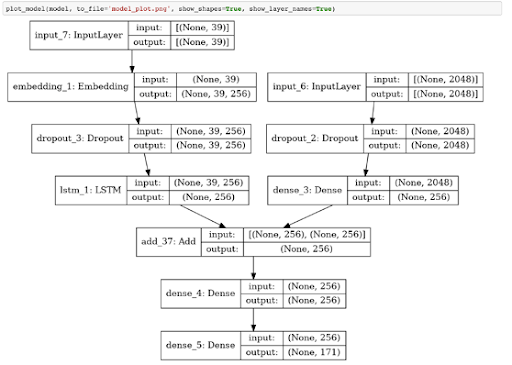
\includegraphics[width=\linewidth]{modelsummary.png}}
\caption{Model Plot}
\label{fig9}
\end{figure}


% RESULTS SECTION
\section{Results}
We started training our model after compiling it and extracting features. Our model's performance did not match our expectations. The categorical accuracy stayed at 100 percent, indicating that the model was not learning. This isn't what we wanted; we wanted our model to generalize rather than memorize interactions. However, we realize that our model didn't have a broad training set because of the lack of descriptions in our text file, which only had one description per picture. Moving forward, we hope to utilize a larger training dataset and analyze our model’s performance. 

% CREATES IMAGE FIGURE
\begin{figure}[htbp]
\centerline{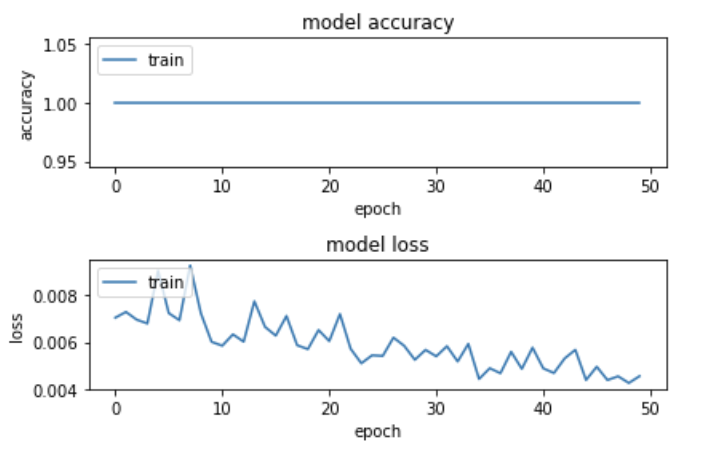
\includegraphics[width=\linewidth]{modelaccuracy.png}}
\caption{Loss and Accuracy History}
\label{fig10}
\end{figure}

We wanted our model to produce images with the expected captions at the top, as previously mentioned. However, we were unable to confirm whether our model completed the task we expected due to a code error that we were unable to debug in time. We think perhaps our model is undertrained. Our results do not show if the captions generated by our model are in the form of a readable text. 

To test the model, we came across various techniques that could be used to compare the actual text description as compared to the caption outputted by the network. We wanted to be able to visualize the results by creating a function that would loop through a certain number of captions and decode the captions. We would have then used this to compare the caption predictions to the actual text file. 

% DISCUSSION SECTION
\section{Discussion}

We faced setbacks during the training phase of these models due to technical difficulties, which prevented us from achieving reliable results that we would have otherwise desired. It's difficult to feel satisfied with what we've achieved because of the lack of detailed training background and mistakes at the end of the code. While the model claims to be 100 percent accurate, this appears to be deceptive, possibly due to the fact that our definition data set was not properly prepared. However, we exceed our baseline expectation.

During the process of this project, we ran into difficulties deciding the project's strategy and lost sight of the project's core functions. The initial aim was to follow a tutorial that would enable us to build a model from the ground up. However, various points of view within the team diverged our focus. We looked at a variety of models and methods, but none of them made sense at first, possibly due to a lack of understanding of new concepts. The Flickr 8k dataset was used to train the majority of the models we saw. We considered taking that route at first, but the use of a data set we had been exposed to in class encouraged us to take a closer look at the actual data preparation process. This method appears to be ineffective; not only did it cause problems mapping descriptions, but the lack of variety of descriptions per picture appears to have harmed our model's learning.

Failures should not be confused for a lack of comprehension. While our model did not always produce exactly what was required of it, we were able to achieve our goal of expanding our knowledge of Neural Networks through practical applications of concepts learned in class. If anything, the difficulty of Image Captioning piqued our interest. Although it is simple to train an Artificial Neural Network to identify images, teaching a machine to understand and interpret proper human language is a method that has yet to yield numerous benefits. Moving forward, we plan to continue to debug our code inorder to get our captions to display along with our images. We would also like to test our data using the comparison approach of “Text” vs. “Net” mentioned above. Comapring the predictions of the network with the actual text will allow us to monitor and modify changes in our network needed to increase accuracy. 

In Conclusion, we leveraged our knowledge and research to experiment with Machine Learning. The technologies and approaches we used are essential takeaways that increase our interest and understanding of the functioning and importance of various different types of Neural Networks. Despite the lack of results, we were able to utilize methods to prepare, construct and train an image captioning neural network.  


% REFERENCES
% THIS IS CREATED AUTOMATICALLY
\bibliographystyle{IEEEtran}
\bibliography{References} % change if another name is used for References file

\end{document}
